


 The first phase of the new experiment ($R_\pi$) would optimally need a beam with pion stopping rate of approximately $3\times 10^5$
  at momentum of $75$ MeV/c with $\frac{\Delta p}{p}=1\%$
in  a spot size  approximately 2 cm dia. This would result in $3\times 10^8$ $\pi^+\to e^+ \nu$ events for a 2-year run. For the $\pi^+ \to \pi^0 e^+ \nu$ experiment the  positive pion stop rate would have to be higher, $1-3\times 10^7$, possibly with  a larger momentum bite e.g. $\frac{\Delta p}{p}=3-5\%$ and using higher pion momentum. This would result in $\geq2\times 10^6$ $\pi^+ \to \pi^0 e^+ \nu$ events for a 4-year run. 

 At present there is only one existing TRIUMF beam possibility, M9A,  that could provide the necessary pion flux but it is apparently fully committed to the condensed matter program. A preliminary investigation of other possibilities was done independently by a TRIUMF technical panel\cite{PIBEAM}. Among the alternatives considered, the most attractive possibility appears to be provision of  a new pion production target (T1.5) and beam line (M13') at a location between the present T1 and T2 production targets as shown in fig.\ref{fig:T1A}. The estimated cost for providing these facilities was $\$8-10$M.
 
\begin{figure}[h!]
\centering
\vspace{-20mm}
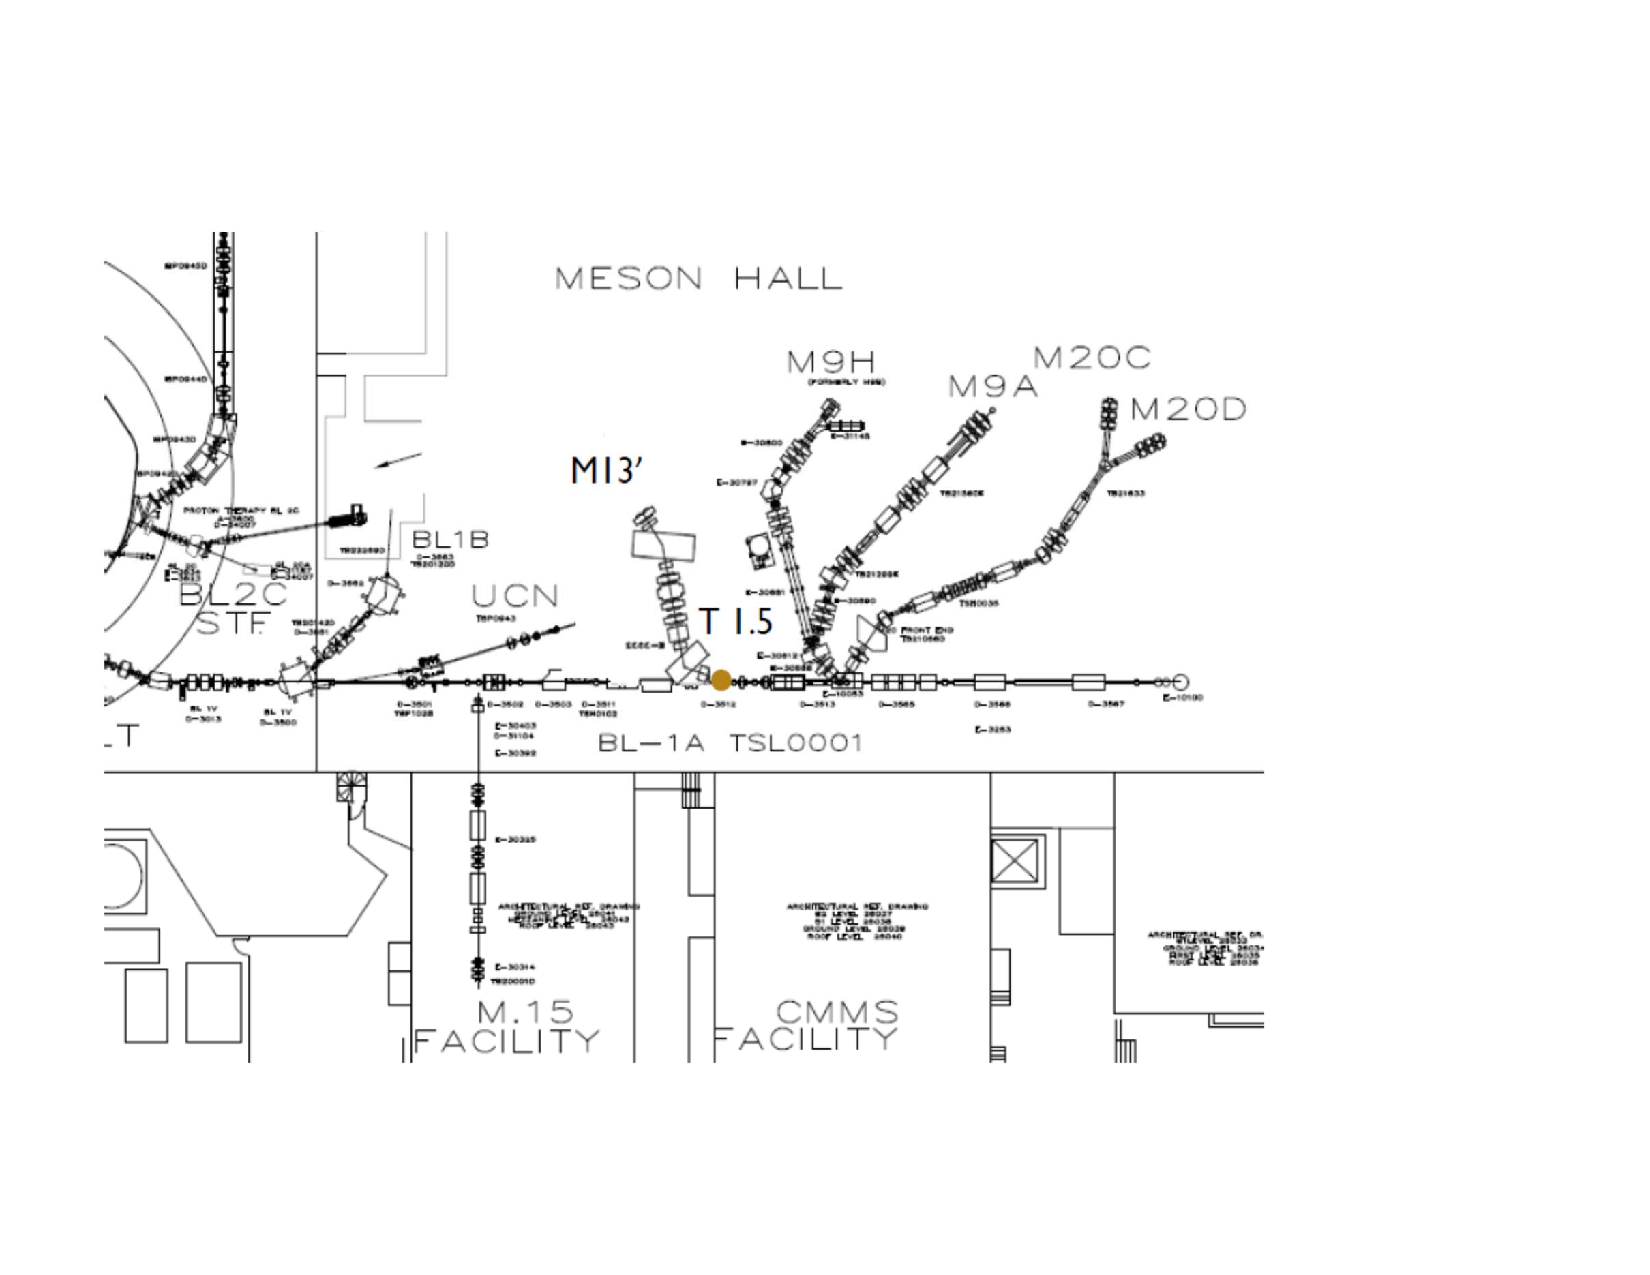
\includegraphics[scale=0.6]{sections/figures/T1.5M13'.pdf}
\vspace{-15mm}
\caption{Schematic concept for T1.5 and M13’, a short pion beam line in the current M11 area\cite{PIBEAM}}
\label{fig:T1A}
\end{figure}

The performance of a new M13' beam line may be estimated by considering a design like the PIE5\cite{PIE5} beam at PSI which has a solid angle acceptance of 150 msr, at 175 deg. take-off. Based on M13 flux measurements\cite{M13E}, it is estimated that a  pion flux of $\geq10^7/s$ could be obtained using a 4 cm thick Be production target. Such a beam line would meet the requirements of the new rare pion decay program discussed here and provide capabilities at TRIUMF for future  experiments involving positive and negative pions and muons. It would provide the highest fluxes at TRIUMF of surface muons for studies such as high precision Michel parameters, searches for $\mu \to e a$, muSR, and others.